%! Author = Dean
%! Date = 12/16/2023


\chapter{Neuronske mreže}\label{ch:neuronske-mreze}

Neuronske mreže čine podskup strojnog učenja i predstavljaju temelj algoritama dubokog učenja.
Inspiracija za strukturu i način rada neuronskih mreža crpi se iz ljudskog mozga pokušavajući oponašazi biološke neurone i njihovu međusobnu komunikaciju.


\section{Umjetni neuron}\label{sec:umjetni-neuron}
Prvi model umjetnog neurona je razvijen od strane Warrena McCullocha i Waltera Pittsa, poznat kao McCulloch-Pitts
model umjetnog neurona. Ovaj model oponaša funkcionalnost biološkog neurona, gdje ulazni signali utječu na odluku neurona o tome hoće li
se on aktivirati ili ne
McCulloch-Pitts model umjetnog neurona sastoji se od \textit{n} ulaznih značajki ili signala, označenih s $x_1, x_2, \dots, x_n$, te njihovim pripadajućim težinama $w_1, w_2, \dots, w_n$ koje određuju važnost pojedinih informacija.
\FloatBarrier
\begin{figure}[h]
    \centering
    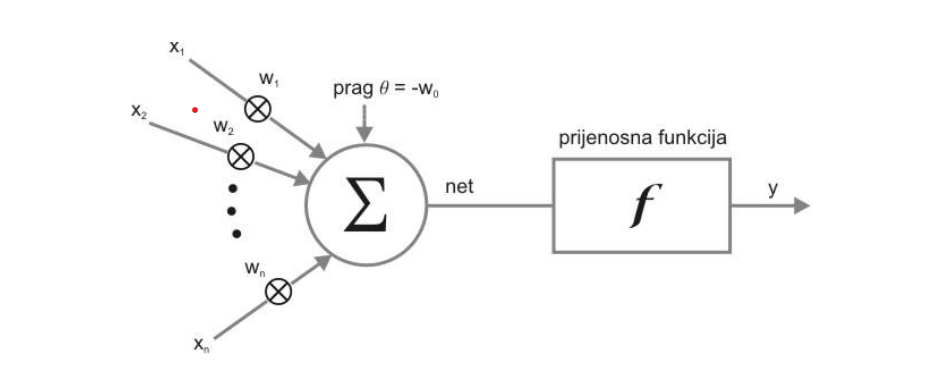
\includegraphics[width=0.8\textwidth]{images/Umjetni_neuron}
    \caption{McCulloch-Pitts model umjetnog neurona%
    \protect\footnotemark}
    \label{fig:slika1}
\end{figure}
\FloatBarrier
\footnotetext{\url{https://www.fer.unizg.hr/_download/repository/UmjetneNeuronskeMreze.pdf}}

Težinska suma neurona \emph{net} se izračunava kao suma ulaznih značajki
\[ net = x_0*w_0 + x_1*w_1 + \dots + x_n*w_n \]
Takozvana vrijednost praga \emph(bias), označena kao $w_0$, koristi se kako bi se odredilo kada će neuron biti aktivan ili ne
Dok nam $x_0$ služi samo radi lakšeg matematičkog zapisa, on je uvijek postavljen na 1.
Znajući sve ovo sad možemo težinsku sumu napisati kao
\[ net = \sum_{i=0}^{\n} w_0*x_0 \]
Drugi način težinske sume koristi vekotorski oblik
\[ net =\vec{w}^T \cdot \vec{x} \]
Na kraju \textit{net} propustimo kroz takozvanu aktivacijsku funckiju \textit{f} koja će nam dati izlaz.

\subsection{Aktivacijska funkcija}\label{subsec:aktivacijska-funkcija}
Aktivacijska funkcija je funkcija koja nam daje izlaz neurona na temelju težinske sume.
Glavna uloga aktivacijske funkcije je ta što ona odlučuje hoće li neuron biti aktivan ili ne ili bolje rečeno hoće neuron u toj situaciji biti
važan u ulozi predikcije.
Najjednostavnija moguća aktivacijska funkcija je funkcija identiteta
\[ f(\textit{net}) = net \]
Danas najčešće korištene aktivacijske funkcije us sigmoidalna u ReLU.
Sigmoidalna funkcija je definirana kao:
\[ f(\textit{net}) = \frac{1}{1 + e^-net} \]
\FloatBarrier
\begin{figure}[h]
    \centering
    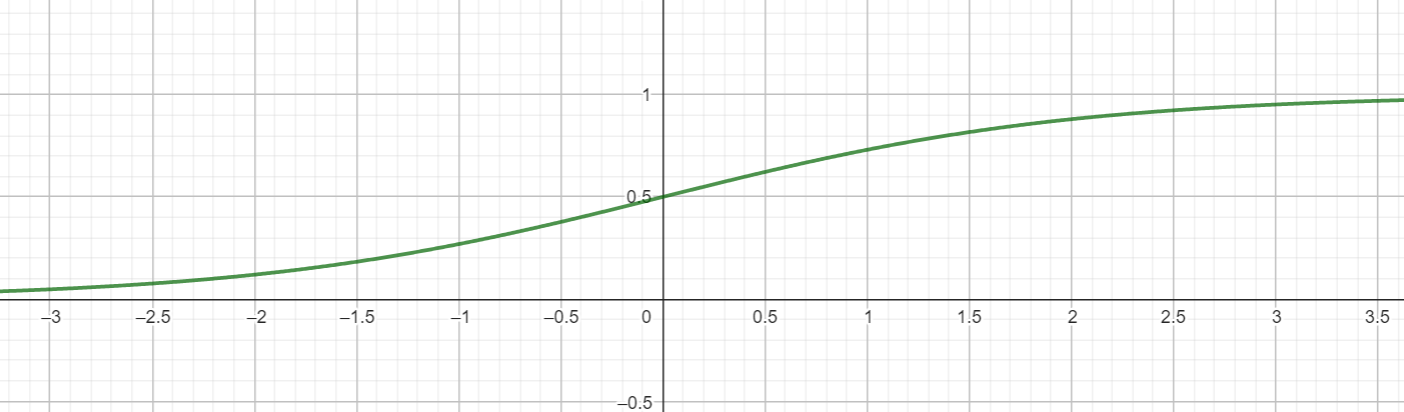
\includegraphics[width=0.8\textwidth]{images/Sigmoid}
    \caption{Sigmoidalna funkcija}
    \label{fig:slika2}
\end{figure}
\FloatBarrier
Kodomena sigmoidalne funkcije je (0, 1) gdje će za jako velike vrijednosti težiti ka 1 a za jako male vrijednosti težiti ka 0.
ReLU aktivacijska funkcija je definirana kao:
\[ f(\textit{net}) = \max(0, \textit{net}) \]
\FloatBarrier
\begin{figure}[h]
    \centering
    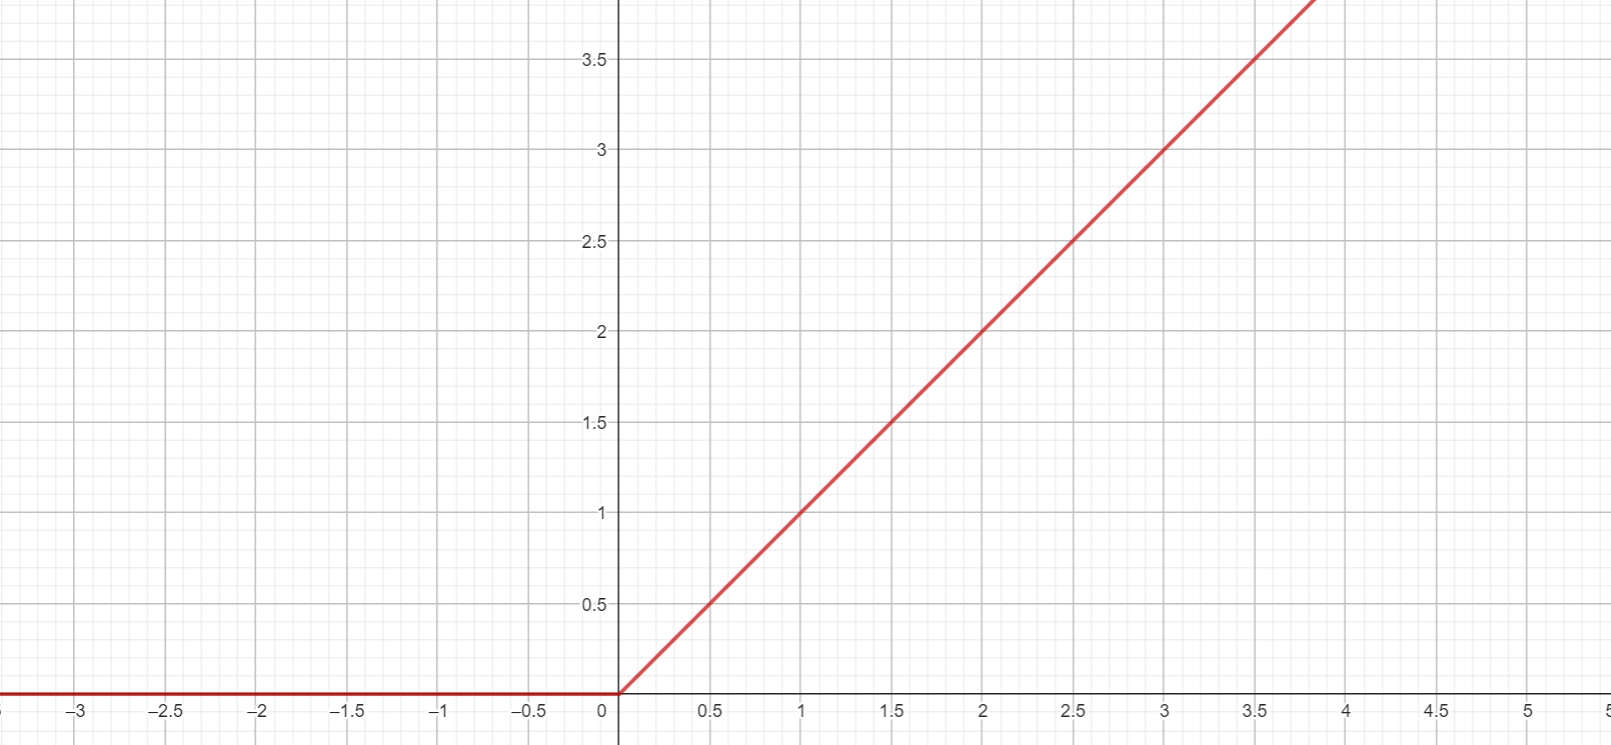
\includegraphics[width=0.8\textwidth]{images/ReLU}
    \caption{ReLU}
    \label{fig:slika3}
\end{figure}
\FloatBarrier


\section{Višeslojne neuronske mreže}\label{sec:viseslojne-neuronske-mreze}

\subsection{Struktura mreže}\label{subsec:struktura-mreze}
Način na koji su neuroni međusobno povezani i organizirani u mreži određuju njezinu arhitekturu te razlikujemo 4 osnovne arhitekture:

\begin{enumerate}
    \item aciklička mreža
    \item mreža s povratnom vezom
    \item lateralno povezana mreža
    \item hibridne mreže
\end{enumerate}

Aciklička mreža nema povratnih veza između neurona tako da je propagacija signala jednosmjerna.
Kod ovakvih vrsta mreža razlikujemo ulazni sloj neurona, skriveni sloj neurona i izlazni sloj neurona.
Ulazni sloj neurona nemaju ulazne signale odnosno nemaju ulogu neurona već samo propagiraju signal iz ulaznog sloja u prvi skriveni sloj.
Skriveni sloj se sastoji od jednog ili više sloja neurona.
Skriveni slojevi igraju ključnu ulogu u procesu učenja i ekstrakciji značajki iz podataka.
Na kraju, izlazni sloj sadrži rezultat.
\FloatBarrier
\begin{figure}[h]
    \centering
    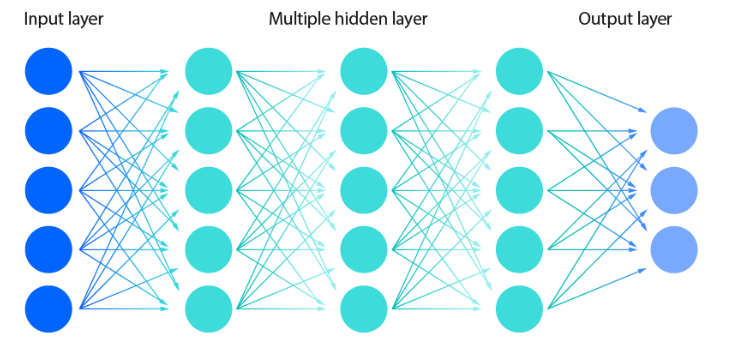
\includegraphics[width=0.8\textwidth]{images/nn-arch}
    \caption{Aciklička mreža
    \protect\footnotemark}
    \label{fig:slika4}
\end{figure}
\FloatBarrier

\footnotetext{\url{https://www.ibm.com/topics/neural-networks}}

Neuronske mreže s povratnom vezom sadrže u svojoj strukturi barem jednu povratnu vezu.
To znači da postoji najmanje 1 ili više čvorova za koje, prateći izlaz neurona kroz sve moguće puteve, nakon konačnog broja koraka ćemo ponovno obići prvobitni čvor.
U ovakvoj arhitekturi, slojeve ne djelimo na ulazne i izlazne, kao što je slučaj kod acikličkih mreža, već govorimo o vidljivim i skrivenim čvorovima.
\FloatBarrier
\begin{figure}[h]
    \centering
    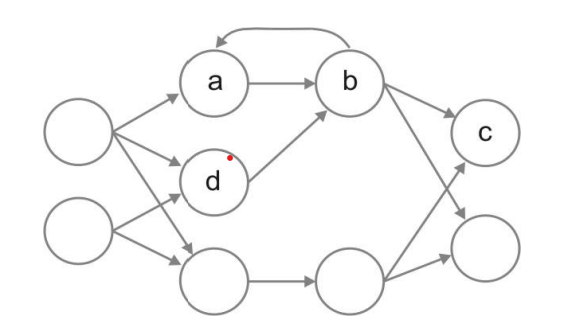
\includegraphics[width=0.8\textwidth]{images/nn-povratna-veza}
    \caption{Mreža s povratnom vezom
    \protect\footnotemark}
    \label{fig:slika5}
\end{figure}
\FloatBarrier
\footnotetext{\url{https://www.ibm.com/topics/neural-networks}}

\pagebreak
Lateralno povezane mreže predstavljaju neuronske mreže gdje neuroni u istom sloju međusobno komuniciraju.
Često se koristi kako bi se omogućila suradnja između neurona kako bi se pojačale određene značajke unutar sloja.
\FloatBarrier
\begin{figure}[h]
    \centering
    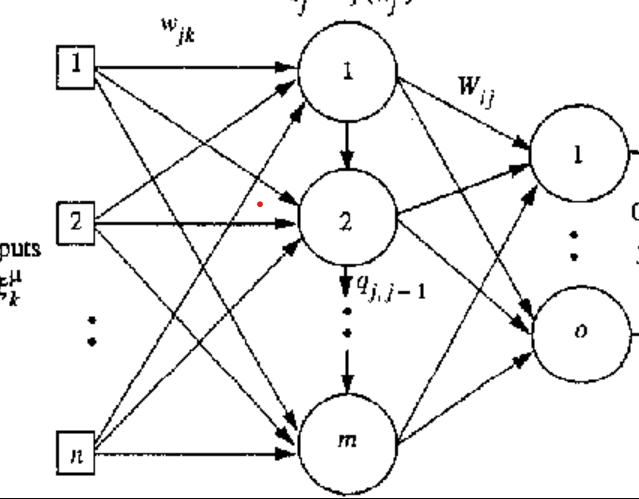
\includegraphics[width=0.8\textwidth]{images/Lateral-connected-nn}
    \caption{Lateralno povezana mreža
    \protect\footnotemark}
    \label{fig:slika6}
\end{figure}
\FloatBarrier
\footnotetext{\url{https://ai.stackexchange.com/questions/34054/what-is-meant-by-lateral-connection-in-the-context-of-neural-networks}}


\section{Backpropagation}\label{sec:backpropagation}
Backpropagation ili postupak propagacije pogreške unatrag je postupak učenja neuronskih mreža koji se temelji na učinkovitom izračunu svih parcijalnih derivacija
i njihovoj primjeni na određivanje iznosa kojim korigiramo svaku od težina.
Algoritam koristi metodu gradijentnog spusta kako bi minimizirao nastalu pogrešku.
Za neuronsku mrežu koja u izlaznom sloju ima \textit{k} izlaznih neurona i za skup za učenje \textit{D}, ukupna empirijska pogreška iznosi:
\begin{align*}
    E(\vec{w}) &= \frac{1}{2N} \sum_{d \in D} \sum_{k \in K} (t_{kd} - o_{kd})^2
\end{align*}
gdje je $t_{kd}$ ciljna ili očekivana vrijednost izlaza, a $o_{kd}$ je stvarna izlazna vrijednost, odnosno vrijednost izlaza neurona.
Algoritam propagacije pogreške unatrag je sljedeći:
\begin{enumerate}
    \item Postavimo početne težine na neke slučajno odabrane vrijednosti
    \item Ponavaljamo postupak dok nije zadovoljen uvjet zaustavljanja
    \begin{itemize}
        \item Postavimo podatke za primjer \textit{i} na ulaz mreže
        \item Izračunamo izlaze svih neurona u svakom sloju
        \item Odredimo pogrešku \textit{i}-tog neurona na izlaznom sloju prema sljedećem izrazu
        \begin{align*}
            \delta_{i}^{K} &= o_{s,i} \cdot (1 - o_{s,i}) \cdot (t_{s,i} - o_{s,i})
        \end{align*}
        gdje nam izraz $o_{s,i}$ * (1 - $o_{s,i}$) označava parcijalnu derivaciju prijenosne funkcije, koja je u ovom primjeru sigmoidalna prijenosna funkcija.
        Izraz ($t_{s,i}$ - $o_{s,i}$) odgovara razlici ciljne i dobivene vrijednosti.
        \item Nakon toga se vraćamo sloj po sloj prema početku neuronske mreže odnosno ulaznom sloju.
        Sada je potrebno za svaki neuron \textit{i} u svakom sloju \textit{k} izračunati njegovu pogrešku.
        To radimo pomoću sljedećeg izraza:
        \begin{align*}
            \delta_{i}^{(k)} &= y_{i}^{k} \cdot (1 - y_{i}^{k}) \left(\sum_{d \in D} w_{i,d} \cdot \delta_{d}^{k+1}\right)
        \end{align*}
        Opet prepoznajemo derivaciju sigmoidalne prijenosne funkcije, a drugi dio izraza odgovara težinskoj sumi pogrešaka neurona kojem on šalje svoj izlaz.
        Bolje rečeno zbraja sve pogreške neurona na čiji ulaz utječe trenutni neuron pomnožen s težinskim faktorom.
        Težinski faktor pokazuje koliko je taj neuron utjecao na iznos pogreške za neuron \textit{s}.
        \item Nakon toga radimo korekciju tezine $w_{i,j}^k$ prema izrazu:
        \begin{align*}
            w_{i,j}^{(k)} \leftarrow w_{i,j}^{(k)} + \eta \cdot y_{i}^k \cdot \delta_{j}^{k+1}\right)
        \end{align*}
        gdje nam je \textit{$\eta$} stopa učenja, \textit{$y_{i}^k$} izlaz neurona i u k-tom sloju, a \textit{$\delta_{j}^{k+1}$} pogreška neurona u sljedećem sloju
    \end{itemize}
\end{enumerate}
Kao što se može vidjeti, naziv algoritma je prikladan jer prvo moramo odrediti izlaz mreže, a nakon toga idemo od izlaznog sloja prema ulaznom sloju i računamo pogrešku neurona u svakom sloju od izlaznog prema ulaznom sloju te korigiramo težine.